

% TODO: NACH TODO SUCHEN!!!!!!!!!!!!!!!!!!!!!!!!!!!!!!!!!!!!!!!!!!!!!!!!!!!!!!!!


\section{Technische Hintergründe}

\subsection{Geschichte des Ext-Dateisystems}

% TODO: AUCH GLEICH BLOG POST! mit paar screenshots vielleicht?

Das sogenannte \ac{ext} war das Erste einer Reihe von Dateisystemen welches speziell für Linux entwickelt wurde und damals das minix-Dateisystem ablöste. \ac{ext} in Version 1 ist mittlerweile allerdings veraltet und wird in aktuellen Linux-Distributionen nicht mehr verwendet. Ext3 ist die neuere Variante, bleibt von Grund auf jedoch exakt gleich wie Ext2, führt jedoch \textit{file system journaling} ein. Die folgenden Varianten sind aktuell noch gängig und werden aktiv eingesetzt:

\begin{itemize}
	\item ext2 - Führte separate Zeitstempel für Dateizugriffe, Inode- und Datenmodifikation ein. Bringt keine Unterstützung für journaling.
	\item ext3 - Führte journaling ein (und ist required!)
	\item ext4 - Aktuelle Version. Unterstützung für fast fsck, native filesystem encryption, journaling, jedoch auch für non-journaling
\end{itemize}

\subsection{Basics}

Das Ext-Dateisystem verwendet Blöcke als Basiseinheit zum Speichern von Daten \cite{Ext2.07.01.2022}, ähnlich wie Cluster in FAT- und NTFS-Dateisystemen. Ein Block kann 1024, 2048 oder 4096 Bytes groß sein. Sogenannte \textit{Inodes }(Index-Nodes) werden zum Speichern von Metadaten verwendet, Blockgruppen zur optimierten logischen Strukturierung, Verzeichnisse um hierarchische Strukturen darstellen zu können, Block- und Inode-Bitmaps um allokierte Blöcke und Inodes zu kennzeichnen, sowie Superblöcke um allgemeine Informationen des Dateisystems zu speichern. Kopien von wichtigen Datenstrukturen wie z.B. den Superblöcken werden redundant vorgehalten und alle Daten welche mit Dateien assoziiert werden, sind aus Gründen der Performance gut lokalisiert\cite{Carrier.06.01.2022}.

\begin{figure}[H]
	\centering
	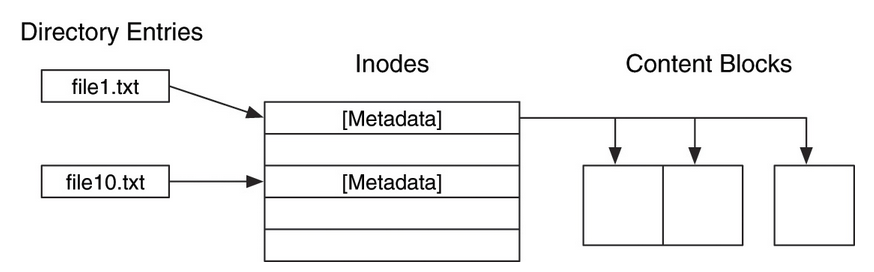
\includegraphics[width=12cm,keepaspectratio=true]{pictures/ext1.png}
	\caption{
		Zusammenhang zwischen Verzeichniseinträgen, Inodes und Inhaltsblöcken \cite{Carrier.06.01.2022}
	}
	\label{fig:ext1}
\end{figure}

Abbildung \ref{fig:ext1} zeigt den Zusammenhang zwischen Verzeichniseinträgen, Inodes und Inhaltsblöcken. Für jede Datei (und für jedes Verzeichnis) existiert eine Inode, welche dazugehörige Metadaten, sowie Referenzen auf die Blöcke mit dem tatsächlichen Inhalt speichert.

\begin{figure}[H]
	\centering
	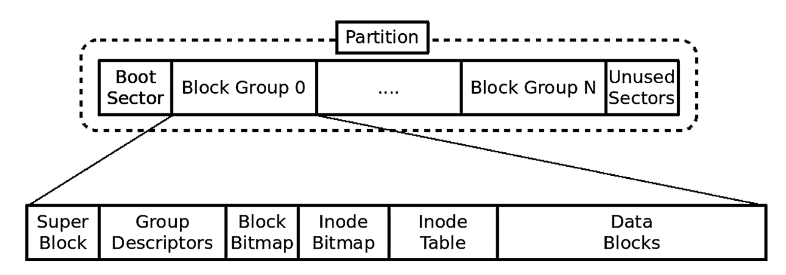
\includegraphics[width=12cm,keepaspectratio=true]{pictures/layout.png}
	\caption{
		Layout des Dateisystems \cite{AnalysisExt4.07.01.2022}
	}
	\label{fig:layout}
\end{figure}

Abbildung \ref{fig:layout} enthält eine graphische Darstellung des Layouts eines Ext-Dateisystems. Die Partition ist in Blockgruppen aufgeteilt und jede Blockgruppe enthält einen Superblock (optional), Group-Descriptors, die Block- und Inode-Bitmap, die Inode-Tabelle sowie die Datenblöcke. Auf diese Aufteilung innerhalb der Blockgruppen wird nun in den folgenden Unterkapiteln näher eingegangen.

\subsubsection{Superblöcke}

Da wir in den praktischen Beispielen (s.u.) ein Ext3 System auf einem USB Stick erstellt haben und dieser keinen OS Kernel enthält, befindet sich auf unserem Stick auch kein Boot-Code. Dieser würde sich sonst in den ersten 1024 Bytes befinden. Der \textit{Superblock} befindet sich ab Offset 1024 des Dateisystems und hat eine Größe von 1024 Bytes, obwohl nicht alle davon verwendet werden. Hier könnte man somit leicht Daten verstecken. Er enthält Basisinformation wie die Blockgröße (z.B. 4096 Byte), die totale Anzahl an Blöcken, die Anzahl an Blöcken pro Gruppe, die Anzahl an Inodes per Blockgruppe, den Volume-Name, den letzten Schreibzugriff, die letzte Mountzeit sowie den Pfad in dem das Dateisystem zuletzt gemounted war. Abbildung \ref{fig:superblock} zeigt eine simple Analyse des Superblocks auf unserem USB Stick.

\begin{figure}[H]
	\centering
	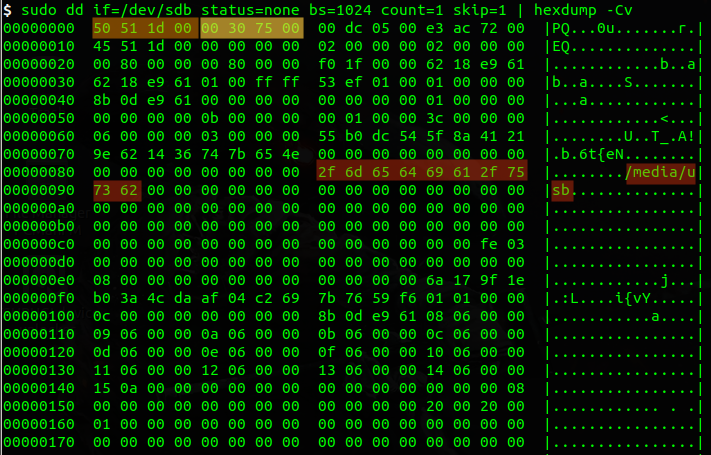
\includegraphics[width=12cm,keepaspectratio=true]{pictures/superblock.png}
	\caption{
		Analyse des Superblocks
	}
	\label{fig:superblock}
\end{figure}

Die ersten 4 Bytes repräsentieren die Anzahl an Inodes: \cite{Ext2.07.01.2022}:\\
\textbf{50 51 1d 00 -> Little endian -> 00 1D 51 50 ergibt 1921360 Inodes}(Vergleiche mit Abbildung \ref{fig:createfs}).\\\\
Die zweiten 4 Bytes repräsentieren die Anzahl an Blöcken:
\textbf{00 30 75 00 => Little endian => 00 75 30 00 = ergibt 7680000 Blöcke}. \\

In der Abbildung ist außerdem noch der Pfad, in welchem das Dateisystem zuletzt gemounted war, markiert: \textbf{/media/usb}.

\subsubsection{Block Group Descriptor Tables}

Im Block nach dem Superblock folgt die Group-Descriptor-Tabelle. Diese beschreibt wo sich Daten wie z.B. die Inode-Tabelle oder die Bitmaps innerhalb einer Blockgruppe befinden. 


\subsubsection{Block- und Inode-Bitmaps}

Die Block- und Inode-Bitmaps speichern den Allokationsstatus von Blöcken, sowie Inodes innerhalb der Blockgruppe. Sie geben also an, welche Blöcke- bzw Inodes innerhalb der Gruppe belegt sind und welche nicht. Jedes Bit repräsentiert hier den Status eines Blocks wobei "1" bedeutet, der Block ist verwendet, "0" bedeutet der Block ist frei bzw. verfügbar. Die Inode-Bitmap funktioniert ähnlich, mit dem Unterschied dass die Bits hier auf den Allokationsstatus einer Inode-Tabelle verweisen.

\subsubsection{Die Inode-Tabelle}

Die Inode-Tabelle wird verwendet um jedes Verzeichnis, jede Datei, symbolischen Link oder Spezialdatei zu beschreiben. Die folgenden Metadaten werden u.a. in den Inodes gespeichert:

\begin{itemize}
	\item Dateigröße
	\item Speicherort (sog. Blockpointer)
	\item Eigentümer (Linux User-Ids)
	\item Gruppe (Linux Group-Ids)
	\item Dateityp
	\item Berechtigungen
	\item Zugriffs- und Änderungs- und Löschzeitpunkt (Gespeichert als typische UNIX-Zeitstempel, also die Nummer an Sekunden seit dem 1. Januar 1970 UTC)
\end{itemize}

Der Dateiname wird nicht in Inodes gespeichert. Eine Datei kann ein Socket, ein Puffer, ein symbolischer Link oder eine normale Datei sein.

In einer Inode befinden sich vordefinierte Datenstrukturen um auf die ersten 12 Blöcke zu referenzieren, welche die Daten der Datei enthalten (\textit{Blockpointer}). Außerdem gibt es weitere Pointer auf Blöcke, die bei größerem Dateiinhalt (> 48KB bei Blocksize 4096) dann einfach weitere Pointer zu weiteren Datenblöcken enthalten.

\subsubsection{Datenblöcke}

Als letztes innerhalb einer Blockgruppe folgen die Datenblöcke, dessen Adressen innerhalb der Inodes gespeichert werden. Hier befinden sich die tatsächlichen Daten.


\subsection{Praktische Beispiele}

Alle praktischen Beispiele zu diesem Dokument wurden unter der \href{https://tsurugi-linux.org/}{Tsurugi Linux-Distribution}  (Version 5.14.6) auf einem 32GB USB Stick durchgeführt und hier völlig transparent, je nach Kontext, präsentiert und sollten somit unter allen gängigen Linuxsystemen 1-zu-1 nachgemacht werden können. 

\begin{lstlisting}[language=bash]
$ uname -a
Linux lab 5.14.6-tsurugi #1 SMP Mon Sep 20 21:45:06 CEST 2021 x86_64 x86_64 x86_64 GNU/Li
\end{lstlisting}  

\newpage
	
Als erstes wurde der USB Stick mit dem Ext3 Dateisystem frisch formatiert:

\begin{lstlisting}[language=bash]
# find mounted devices and their paths:
lsblk

# unmount the device: (The usb stick here is "/dev/sdb")
sudo umount /dev/sdb

# Create the filesystem:
sudo mkfs -t ext3 /dev/sdb
\end{lstlisting}  

\begin{figure}[H]
	\centering
	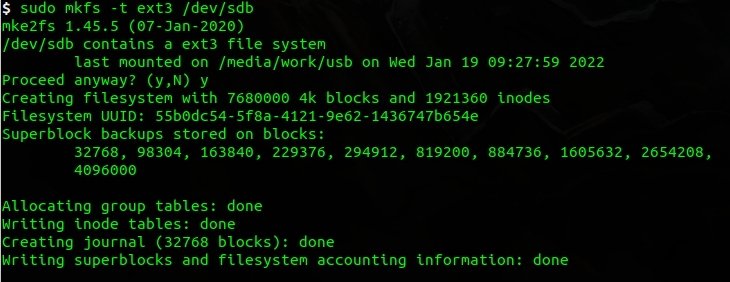
\includegraphics[width=12cm,keepaspectratio=true]{pictures/createfs.png}
	\caption{
		Erstellen eines EXT3 Dateisystems auf einem USB Stick
	}
	\label{fig:createfs}
\end{figure}

Im Abbildung \ref{fig:createfs} ist zu sehen wie das Dateisystem auf dem USB Stick unter \textit{/dev/sdc} erstellt wird. Es werden 7680000 4KB Blöcke mit 1921360 Inodes erstellt (32GB). Für das Dateisystem wird eine \ac{uuid} generiert, ein Journal erstellt, sowie die Blöcke in denen sich die Superblock-Backups befinden, ausgegeben.


\subsubsection{Erstellen von Dateien}

Folgendes Listing erzeugt eine Datei:

\begin{lstlisting}[language=bash]
# Asumming the fs is mounted on /media/usb
cd /media/usb
touch mydocument.txt
echo "Hallo welt." > mydocument.txt
\end{lstlisting} 

Mit Hilfe des Kommandos \textit{ls -li} können wir uns die Inode-ID ausgeben lassen um diese dann mit Hilfe des SleuthKit (\cite{Sleuthkit.07.01.2022}) Kommandos \textit{istat} näher zu betrachten. Abbildung \ref{fig:istatman} zeigt die Ausgabe der Manual-Page für das Tool.

\begin{figure}[H]
	\centering
	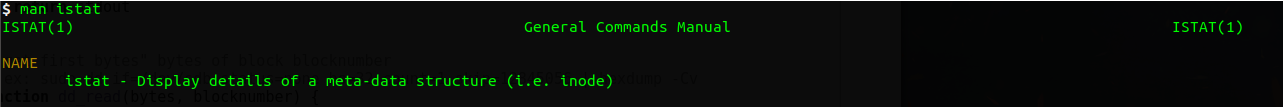
\includegraphics[width=12cm,keepaspectratio=true]{pictures/istat-man.png}
	\caption{
		Manual page \textit{istat}
	}
	\label{fig:istatman}
\end{figure}


\begin{figure}[H]
	\centering
	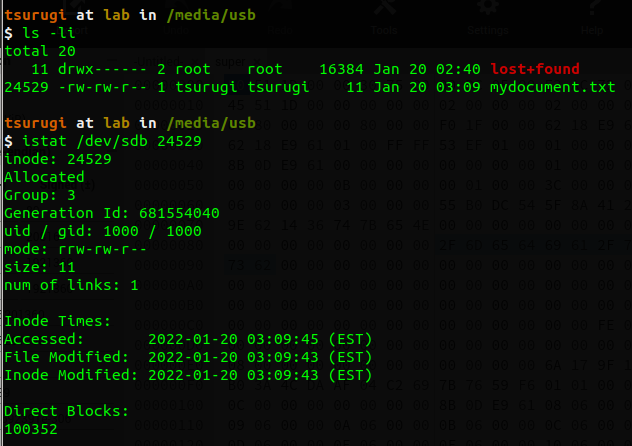
\includegraphics[width=12cm,keepaspectratio=true]{pictures/inode-stats.png}
	\caption{
		Informationen einer Inode
	}
	\label{fig:inodestats}
\end{figure}

Wir sehen in Abbildung \ref{fig:inodestats}, dass unsere zuvor erstellte Datei \textit{mydocument.txt} zur Inode 24529 gehört. Sie befindet sich in Blockgruppe 3, hat eine Größe von 11 Bytes (Inhalt: \textit{Hallo welt.}) und der Inhalt der Datei befindet sich in Block Nummer 100352.

Mit Hilfe von \textit{dd} wollen wir uns nun den Inhalt des Blocks 100352 ansehen, um zu verifizieren ob dort auch die Daten unserer Datei liegen:

\begin{figure}[H]
	\centering
	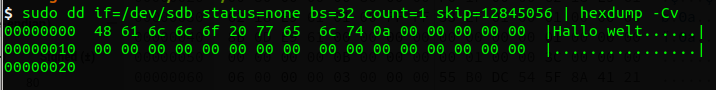
\includegraphics[width=12cm,keepaspectratio=true]{pictures/getfilecontent.png}
	\caption{
		Rohen Inhalt eines Blocks mit \textit{dd} auslesen
	}
	\label{fig:getfilecontent}
\end{figure}

Da jeder Block in unserem Dateisystem 4096 Bytes groß ist, beginnt der Inhalt dieser Datei an Byteoffset 411041792 (Blocknummer x Blockgröße). Wir kopieren mit \textit{dd} immer 32 Byte, müssen daher mit Hilfe des \textit{skip}-Arguments angeben, ab wann wir mit dem Kopieren starten wollen (411041792/32 = 12845056). Und siehe da, der Inhalt der Datei wird korrekt ausgegeben!

\subsubsection{Löschen von Dateien}

Wir löschen die Datei mit folgendem Kommando:

\begin{lstlisting}[language=bash]
rm -rf mydocument.txt
\end{lstlisting} 

Wir wissen noch die Inode ID 24529. Abbildung \ref{fig:istatafterdelete} zeigt die Analyse dieser Inode mittels \textit{istat} nach dem Löschen der Datei:

\begin{figure}[H]
	\centering
	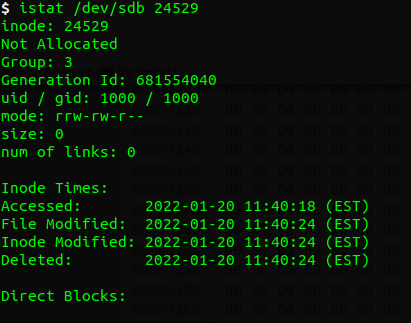
\includegraphics[width=12cm,keepaspectratio=true]{pictures/istatafterdelete.png}
	\caption{
		Inode-Inhalt nach dem Löschen auslesen
	}
	\label{fig:istatafterdelete}
\end{figure}

Die Inode gilt nun nicht mehr als allokiert (\textit{Not Allocated}), die Dateigröße wurde auf 0 Byte gesetzt und die Referenz zum Inhaltsblock entfernt (Blockpointers zeroed). Außerdem kam ein \textit{Deleted}-Datensatz hinzu. Dennoch können wir immer noch die Daten der vorherigen Blocknummer mittels \textit{dd} wie oben beschrieben auslesen und bekommen den Inhalt der Datei. Es wird also nicht der Inhalt, sondern nur die Referenz in der Inode gelöscht und somit auch der Speicherplatz freigegeben. Dieser kann nun zu späterem Zeitpunkt überschrieben werden.

\newpage

\section{Forensische Analyse des EXT3 Dateisystems}

\subsection{Erstellen einer forensischen Arbeitskopie}

Normalerweise würden wir vor einer Analyse immer zuerst eine forensische Arbeitskopie erstellen. Aus Gründen der Einfachheit wird hier jedoch darauf verzichtet und bei sämtlichen Analysen direkt auf das Blockdevice (\textit{/dev/sdb}) zugegriffen.

Folgende Kommandos könnten verwendet werden:

\begin{lstlisting}[language=bash]
$ sudo dd if=/dev/sdb of=usb.dd bs=512 conv=noerror,sync status=progress

# dc3dd is a forensics extension of dd (e.g. hash based verification integrated)
dc3dd if=/dev/sdb hof=/path/to/my/backup.raw hash=sha256
\end{lstlisting}


\subsection{Forensische Konzepte zur Auswertung}

Im diesem Kapitel werden einige Konzepte zur Auswertung von Ext-Dateisystemen vorgestellt. Wir wissen, dass im Superblock wichtige Informationen über das Dateisystem gespeichert sind und können somit dort ansetzen. Sollte der Superblock korrupt sein, ist es auch relativ einfach nach Backups zu suchen um dann diese zu verwenden.

Wir könnten den Superblock wie oben bereits beschrieben manuell analysieren, mit Hilfe des Tools \textit{fsstat} ist es  jedoch einfacher, sich grundlegende Information ausgeben zu lassen. Das Tool gibt Metadaten, sowie Inhaltsinformationen aus und anschließend Informationen zu jeder Blockgruppe. Diese Informationen können für weitere Untersuchungen sehr hilfreich sein. Abbildung \ref{fig:fsstat} zeigt die Ausgabe des Tools für unseren USB Stick. Wir sehen z.b. auch, welche Blöcke in welcher Gruppe liegen, eine Information die besonders relevant sein kann.

\begin{figure}[H]
	\centering
	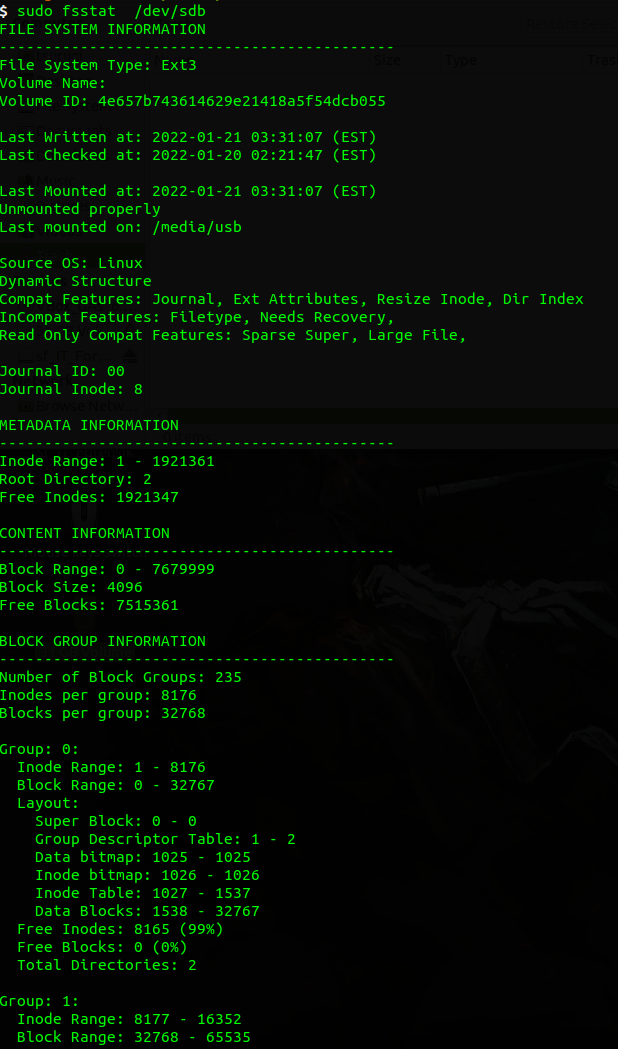
\includegraphics[width=12cm,keepaspectratio=true]{pictures/fsstat.png}
	\caption{
		Ausgabe von fsstat für unseren USB Stick
	}
	\label{fig:fsstat}
\end{figure}

Für die weitere Auswertung von Inhalten, ist es wichtig den Allokationsstatus von Blöcken zu kennen. Ist ein Block belegt, so ist das ein Hinweis darauf, dort verwertbare Daten zu finden. Diesen Allokationsstatus zu finden ist ein 3-Schritte-Prozess (\cite{Carrier.06.01.2022}):

\begin{enumerate}
	\item Feststellen, zu welcher Blockgruppe der Block gehört
	\item Suchen des Eintrags der Gruppe in der Group-Descriptor-Tabelle um festzustellen, wo ihre Block-Bitmap gespeichert ist
	\item Zuletzt wird die Block-Bitmap analysiert und das dem betreffenden Block zugeordnete Bit untersucht. Wenn das Bit gesetzt ist, ist der Block allokiert
\end{enumerate}

Der Allokationsstatus kann auch für das Wiederherstellen gelöschter Dateien hilfreich sein, denn mit dessen Hilfe kann die Suche nach bestimmten Inhalten (z.B. Keywords) auf gewissen Blockgruppen beschränkt werden, was viel Zeit sparen kann. 

Bisher haben wir den Inhaltsbereich analysiert. Ein weiterer Ansatz ist es, den Metadatenbereich zu verwenden. In unserem praktischen Beispiel haben wir bereits gesehen, dass nach dem Löschen einer Datei immer noch die Inode ausgelesen werden kann. Die Größe und Blockreferenz wird zwar gelöscht, dennoch gibt es einen \textit{Deleted}-Datensatz mit dem Zeitstempel der Löschung, sowie weitere oben beschriebenen Informationen sind noch intakt. Diese Informationen in den Inodes können hilfreich für eine weitere Auswertung sein.

Weitere Möglichkeiten der Auswertung basierend auf der Dateinamen- oder Applikationskategorie werden in \cite{Carrier.06.01.2022} beschrieben, darauf wird jedoch hier nicht weiter eingegangen. Abschließend befassen wir uns im nächsten Kapitel mit dem Wiederherstellen gelöschter Dateien. 

\subsection{Wiederherstellen gelöschter Dateien}

Zurück zu unserem Beispiel oben, wir wissen ja noch die Inode ID 24529. Außerdem kennen wir den Inhalt "`Hallo Welt "'. Somit könnten wir als erste Idee zur Auswertung einfach nach dem Inhalt suchen:

\begin{lstlisting}[language=bash]
$ sudo strings /dev/sdb | grep "Hallo"
\end{lstlisting}
 
Dieses Kommando findet zwar den Inhalt noch, obwohl die Datei gelöscht wurde. Das sagt uns aber nichts über den Speicherort  und bei verschlüsselten oder kodierten Inhalten würde uns das auch nicht weit bringen. Außerdem kennen wir normalerweise auch nicht die Inode. Wir benötigen bessere Methoden zur Auswertung und Datenwiederherstellung. Zwei davon werden im Folgenden präsentiert und erläutert.

\subsubsection{File-Carving}

Die Wiederherstellung von Dateien ist bei Ext3-Dateisystemen nicht einfach. Bei Ext2 werden die Inode-Werte nicht gelöscht, wenn die Datei gelöscht wird, so dass die Blockzeiger noch vorhanden sind. Die Zeitwerte werden ebenfalls aktualisiert, wenn die Datei gelöscht wird, so dass man weiß, wann die Löschung erfolgt ist.

Bei Ext3 ist der Zusammenhang zwischen dem Dateinamen und dem Inode noch vorhanden, aber die Blockpointer werden gelöscht. Um die Daten wiederherzustellen, ist es möglich  sog. File-Carving-Techniken anzuwenden. Gruppeninformationen lassen sich aus Performancegründen hier zu unserem Vorteil nutzen. Die Zuweisung von Blöcke in Blockgruppen ist jedoch abhängig vom Betriebssystem, es könnte also auch ein Carving des gesamten Platzes notwendig sein: es kann also ein zeit-intensives Unterfangen sein.

File-Carving bedeutet das Suchen nach bestimmten Mustern (wie z.B. JPEG header Informationen) im rohen Binärdaten und somit das Zusammenfassen von unstrukturierten Inhalten zu einer Datei.
Ein Tool dafür soll hier vorgestellt werden: Foremost \cite{Foremost.07.01.2022}

Foremost ist ein Tool zur Wiederherstellung gelöschter Daten unter Verwendung von gängigen Datei-headern, footern sowie internen Datenstrukturen. Die Config-Datei unter \textit{/etc/foremost.conf} enthält binäre Signaturen zur Erkennung vieler gängiger Dateitypen.\\

Für das praktische Beispiel wurde eine \textit{png}-Datei angelegt und anschließend via \textit{rm} gelöscht. Folgendes Kommando wurde zur Wiederherstellung verwendet:

\begin{lstlisting}[language=bash]
sudo foremost -t jpg,png -v -q -d -b 4096 -i /dev/sdb -o /home/tsurugi/output
\end{lstlisting}

Nach ca. zwei Stunden war \textit{foremost} fertig und hat den Screenshot korrekt wieder hergestellt:

\begin{figure}[H]
	\centering
	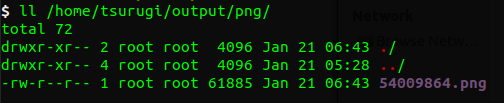
\includegraphics[width=12cm,keepaspectratio=true]{pictures/foremostsuccess.png}
	\caption{
		Das Tool \textit{foremost} speichert wiederhergestellte Dateien im \textit{output} Ordner
	}
	\label{fig:foremostsuccess}
\end{figure}

Eine weitere Methode zur Wiederherstellung gelöschter Daten wird im nächsten Kapitel vorgestellt.

\subsubsection{Das File-Journal}

Das File-Journal wurde in Ext3 eingeführt und stellt die Integrität eines Dateisystems sicher, indem es eine Art Logbuch von Schreibzugriffen speichert. Dies ist u.a. hilfreich bei einem Systemabsturz oder Stromausfall. Mit ein bisschen Glück lassen sich in diesem Journal noch alte Inode-Kopien gelöschter Dateien finden, welche immer noch die Block-Referenzen beinhalten. Durch diesen Ansatz kann der Inhalt wiederhergestellt werden.

Ein Tool zur Automatisierung der Wiederherstellung von Daten in Ext-Dateisystemen, welches auf dem oben beschriebenen File-Journal Ansatz basiert, soll hier abschließend vorgestellt werden: \textit{ext4magic} \cite{Ext4magic.07.01.2022}.
Abbildung \ref{fig:ext4magic} zeigt das Tool in Aktion. Nach erfolgreicher Wiederherstellung wird hier der Inhalt mittels \textit{cat} ausgegeben (Inode 24529).

\begin{figure}[H]
	\centering
	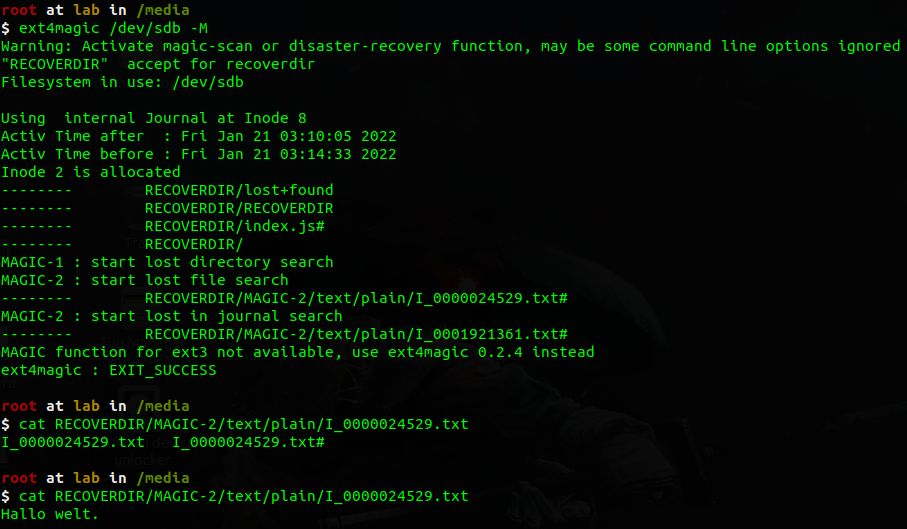
\includegraphics[width=12cm,keepaspectratio=true]{pictures/ext4magic-recovery.png}
	\caption{
		Wiederherstellung gelöschter Daten mit dem Tool \textit{ext4magic} \cite{Ext4magic.07.01.2022}
	}
	\label{fig:ext4magic}
\end{figure}